% Report skeleton (P3). Structure and page budget follow spec.md §9.
% TODO(all): if the organizers publish an official template, move these sections into it unchanged;
%            no margin/font/spacing compression. Body incl. AI statement <= 4 pages; references separate.
% Numbers marked [measured] come from runs/ via shared/*.py; regenerate, never retype.
% Scientific judgments are left as TODO for the team to author (spec §1: "The human team authors the
% final scientific judgments").
\documentclass[11pt]{article}
\usepackage[margin=1in]{geometry}
\usepackage{graphicx,booktabs,amsmath,amssymb,hyperref}
\newcommand{\todo}[1]{\textbf{[TODO: #1]}}

\title{Does Reflection Symmetry Improve Pitching-Wing Wake Forecasts at Unseen Kinematics?}
\author{\todo{team name / members}}
\date{Siderius Hackathon Track 2 --- 21 November 2026}

\begin{document}
\maketitle

% ---------------------------------------------------------------- 0.25 page, owner: all
\begin{abstract}
\todo{one sentence each: question; comparison (A: released CNN, B: + reflection augmentation,
C: B + forecast reflection averaging); result with paired case-level change and interval;
key limitation (12 validation cases, one training seed).}
\end{abstract}

% ---------------------------------------------------------------- 0.45 page, owner: P2
\section{Goal and hypothesis}
The task forecasts 20 future vorticity frames of the wake of a NACA0012 pitching at
$\mathrm{Re}=500$ from 10 past frames and the kinematics $(k, \theta_0, \text{phase})$.
Reflecting $y\to-y$ maps the problem onto itself: vorticity changes sign and the rows flip,
the pitching phase advances by $\pi$ ($\sin$ and $\cos$ of the phase both negate), and
$k$, $\theta_0$ are unchanged. We write $G$ for this map on inputs and $S$ for it on forecasts.

\todo{P2: physical justification of $G,S$ (geometry, motion, boundaries); state that individual
wakes may be deflected/asymmetric, so we test map equivariance $F(Gx)=S(F(x))$, not symmetric states.}

\noindent\textbf{Hypothesis.} B reduces the reflection defect; C enforces it exactly and may improve
forecast accuracy. \textbf{Contradicting evidence:} unchanged or worse paired case-level forecast
NMSE despite better consistency. \todo{predeclared practical tolerance for ``negligible'' gains: \_\_\_}

% ---------------------------------------------------------------- 0.55 page, owner: all
\section{Research trajectory}
\begin{tabular}{p{0.16\linewidth}p{0.2\linewidth}p{0.2\linewidth}p{0.2\linewidth}p{0.14\linewidth}}
\toprule
Run & Why & Change & Result & Next decision \\
\midrule
A\_official & reference/fallback & none (organizer weights) & NMSE 0.2571 [measured] & \todo{} \\
C\_on\_A & cheap symmetry test & mirror averaging at inference & NMSE 0.2562; $\Delta$ $-0.001$, CI $[-0.072,+0.059]$ [measured] & \todo{} \\
B\_s0 & learn symmetry & $p{=}0.5$ reflection augmentation, 40 epochs, 1068\,s & NMSE 0.2094; defect 0.051 vs 0.164 [measured] & \todo{} \\
A\_s0 & matched control & none, local seed 0 & stopped at epoch 3 when the GPU was reassigned; no result & \todo{} \\
C\_from\_B\_s0 & exact consistency & averaging on B & NMSE 0.1856; $\Delta$ vs B $-0.024$, CI $[-0.027,-0.020]$, 12/12 cases [measured] & \todo{} \\
Bplus\_s0 & more data & B with all training windows (3$\times$) & \todo{pending: runs/p3/bplus} & \todo{} \\
\bottomrule
\end{tabular}

% ---------------------------------------------------------------- 1.45 pages, owner: P1/P3
\section{Final model and comparisons}
\textbf{Configurations.} A and B use the released width-64 encoder--decoder, the same seed-0
initialization, windows, optimizer, schedule and epochs; B differs only by per-example reflection of
the full history and all 20 targets with probability 0.5 (independent RNG, so A's window order is
unchanged). C averages the complete forecasts of B on $x$ and $Gx$:
$F_C(x)=\tfrac12\big(F(x)+S(F(Gx))\big)$, which satisfies $F_C(Gx)=S(F_C(x))$ exactly and costs
two forward passes. The statistics head (mean field, spectrum, Strouhal, regime) is untouched.

\textbf{Evaluation.} Official scorer; per-lead NMSE is clipped at 4 \emph{before} averaging (verified
with a synthetic counterexample: 1.5 vs.\ 1.75, \texttt{shared/test\_clip\_order.py}). Paired
case-level differences over the same 12 validation cases with a 2000-resample case bootstrap; the
interval describes case-sampling variability only, not seed noise or a population gain.
Reflection defect $\|F(Gx)-S(F(x))\|^2 / (\|F(x)\|^2+\|F(Gx)\|^2)$, averaged by case.

\begin{table}[h]\centering\scriptsize
% regenerate: shared/results_table.py --out report/results_table ...
\IfFileExists{../runs/p3/final/results_table.tex}{\begin{tabular}{lllrrrrrlrr}
\toprule
Config & Seed & Provenance & NMSE & NMSE$_{20}$ & St err & Utility & Refl.\ defect & Health & Lat.\ (ms) & Train (s) \\
\midrule
A\_official & 0 & organizer checkpoint (reference; not a local run) & 0.2571 & 0.4105 & 0.0701 & 0.7476 & 0.164 & pass & 5.6 & - \\
C\_on\_A & 0 & organizer checkpoint + mirror averaging, no training & 0.2562 & 0.3696 & 0.0701 & 0.7483 & 0.000 & pass & 6.3 & - \\
B\_s0 & 0 & local train, seed 0, reflection aug. p=0.5 & 0.2094 & 0.3144 & 0.0701 & 0.7857 & 0.051 & pass & 5.6 & 1068 \\
C\_from\_B\_s0 & 0 & B\_s0 weights + mirror averaging, no training & 0.1856 & 0.2754 & 0.0701 & 0.8048 & 0.000 & pass & 6.3 & - \\
\bottomrule
\end{tabular}
}{\todo{results\_table.tex not generated yet}}
\caption{Validation results. Utility $=[2\,\mathrm{clip}(1-\mathrm{NMSE})+0.5\,\mathrm{clip}(1-\mathrm{St\,err}/0.3)]/2.5$.
Latency: median batch-1 forward, \todo{device; idle GPU?}.}
\label{tab:results}
\end{table}

\begin{figure}[h]\centering
\IfFileExists{../runs/p3/final/fig1.pdf}{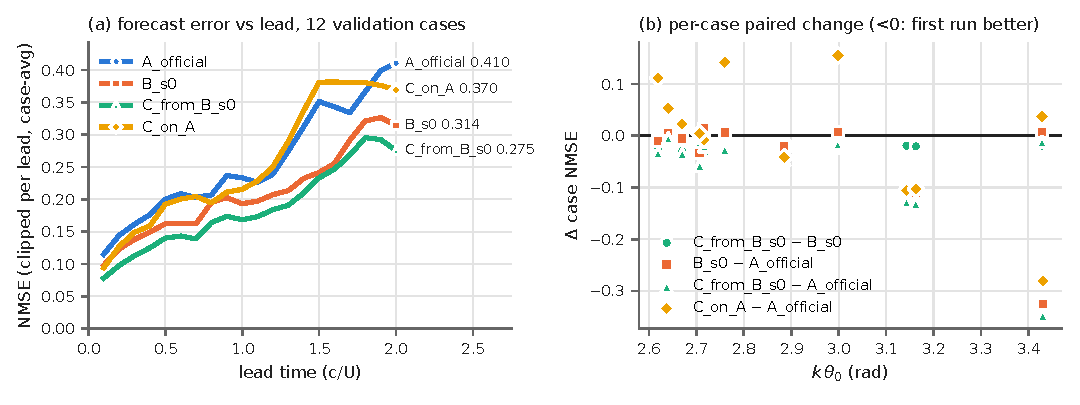
\includegraphics[width=\linewidth]{../runs/p3/final/fig1.pdf}}{\todo{fig1.pdf}}
\caption{(a) Clipped NMSE by forecast lead (cases averaged). (b) Paired per-case change vs.\ $k\theta_0$;
comparisons against A\_official are not matched (organizer checkpoint, no local A).}
\label{fig:lead}
\end{figure}

\textbf{Gates} [measured, \texttt{shared/health\_gate.py} with the task's own health view and the framework
check]. All four configurations pass the shape, finiteness, NMSE$\le1$, \texttt{forecast\_not\_frozen\_in\_time}
(dispersion 0.442, 0.389, 0.460, 0.457 for A\_official, C\_on\_A, B\_s0, C\_from\_B\_s0; floor 0.05) and
latency gates (median batch-1 forward 5.6\,ms single-pass, 6.3\,ms mirror-averaged, NVIDIA H100, measured
while another training job shared the GPU). Statistics outputs are identical between B\_s0 and C\_from\_B\_s0.
Forecast equivariance error $\max|F(Gx)-S(F(x))|$ is exactly 0 for both C models (0.79 and 0.42 relative for
A\_official and B\_s0).

\textbf{Submission.} \todo{P1: selected configuration, submission ID, code revision, ZIP sha256,
reproduction result.}

% ---------------------------------------------------------------- 0.65 page, owner: all (human-authored)
\section{Insights}
\todo{At most three. Each: claim / evidence (table, figure, paired interval) / limitation.
Team-authored; do not let an AI write these judgments.}

\begin{figure}[h]\centering
\IfFileExists{../runs/p3/final/fig2.pdf}{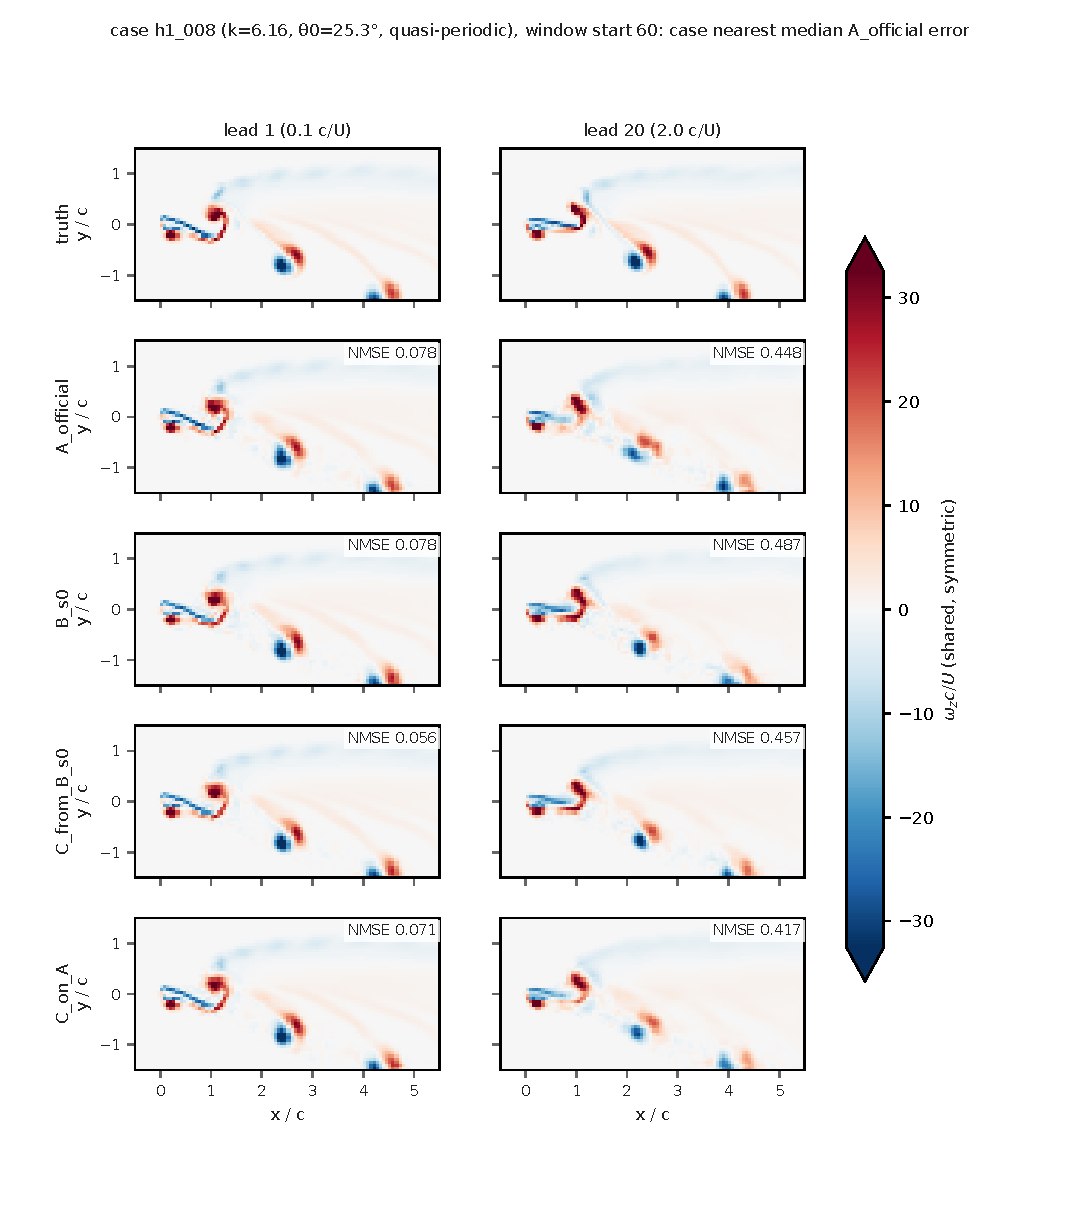
\includegraphics[width=0.85\linewidth]{../runs/p3/final/fig2.pdf}}{\todo{fig2.pdf}}
\caption{Truth vs.\ forecasts at lead 1 and lead 20, first window of the case nearest the median
reference error (selected by rule, not by gain). Shared symmetric colour scale.}
\label{fig:fields}
\end{figure}

% ---------------------------------------------------------------- 0.30 page, owner: all
\section{Limitations and next experiment}
No matched local A (the A\_s0 run stopped at epoch 3), so B vs.\ A compares against the organizer
checkpoint and mixes augmentation with any local-vs-organizer training difference; the C vs.\ B comparison
is matched (same weights). 12 validation cases; one training seed per configuration; model selected on
validation; local validation NMSE is not a leaderboard score; C doubles
inference cost; equivariance is guaranteed for the averaged map, not an improvement in clipped NMSE;
the 10-frame input may omit dynamical state. Next control: \todo{same-cost non-symmetry two-pass
ensemble, or a second matched seed}.

% ---------------------------------------------------------------- 0.35 page, owner: P1
\section{Reproducibility, contributions and AI use}
\todo{exact commands, environment (torch 2.10.0+cu128, NVIDIA H100 80GB), seeds, train-only fitting,
links to code and evidence; roles of each member; verified AI uses (what was generated, how checked).}

\clearpage
\begin{thebibliography}{9}\small
\bibitem{bose2021} Bose et al.\ (2021), pitching--heaving wake transitions. \todo{full ref}
\bibitem{elesedy2021} B.~Elesedy and S.~Zaidi (2021), Provably strict generalisation benefit for equivariant models. \todo{venue}
\bibitem{fromme2025} Fromme et al.\ (2025), equivariant fluid surrogates. \todo{full ref}
\end{thebibliography}
\end{document}
